\ylDisplay{Autod peeglis} % Ülesande nimi
{Tundmatu autor} % Autor
{piirkonnavoor} % Voor
{2007} % Aasta
{P 4} % Ülesande nr.
{1} % Raskustase
{
% Teema: Valgusõpetus
\ifStatement
 Toas on vastasseintes maast laeni tasapeeglid. Kristi veeretab põrandal mänguautot risti peeglitega. Akki märkab ta, et peeglites on palju liikuvaid autosid. Milline on auto teise kujutise kiirus esimese kujutise suhtes kummaski peeglis, kui Kristi lükkab autot ühe peegli poole kiirusega $v = 0,5$ m/s?
\fi

\ifHint
Eimeses peeglis esimene kujutis läheneb temale ja teine kujutis kaugeneb temast. Mõlemad liiguvad kiirusega $v = 0,5$ m/s.
\fi


\ifSolution
Olgu peegel, millele auto läheneb kiirusega $v$, esimene, ning millelt kaugeneb sama kiirusega – teine. Siis esimeses peeglis läheneb esimene auto kujutis mõlemale peeglile kiirusega $v$ ja teises peeglis esimene kujutis kaugeneb mõlemast peeglist kiirusega $v$. Esimene kujutis esimeses peeglis tekitab teise kujutise teises peeglis ja vastupidi. Kuna esimene kujutis esimeses peeglis läheneb kiirusega $v$, siis teine kujutis teises peeglis samuti läheneb kiirusega $v$. Analoogiliselt, kuna esimene kujutis teises peeglis kaugeneb kiirusega $v$, siis teine kujutis esimeses peeglis samuti kaugeneb kiirusega $v$. Kokkuvõttes saime, et esimeses peeglis esimene kujutis läheneb temale ja teine kujutis kaugeneb temast. Järelikult esimeses peeglis eemaldub teine kujutis esimesest kiirusega $2v = 1$ m/s. Teises peeglis aga esimene kujutis kaugeneb temast ja teine kujutis läheneb temale. Järelikult teises peeglis läheneb teine kujutis esimesele kiirusega $2v = 1$ m/s. Näitlikustavatel joonistel on kujutatud olukord hetkel, kui toa laius on $4$ m ning auto asub alghetkel toa keskel (ülemine joonis). Alumisel joonisel on kujutatud olukord $1$ sekundi möödumisel liikumise algusest.
\begin{center}
	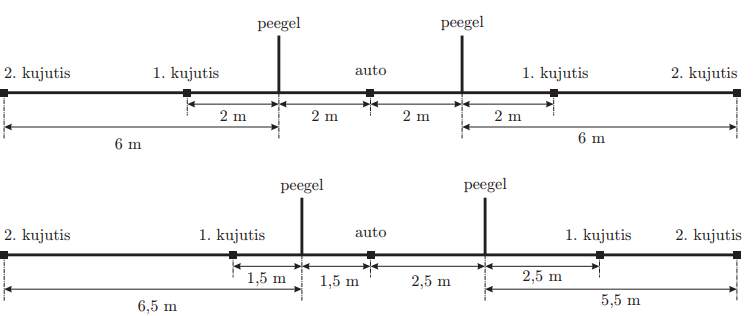
\includegraphics[width=0.5\linewidth]{2007-v2p-04-lah.PNG}
\end{center}
\fi
}
